% =====================================================================
% AUTO-GENERATED from docs/erw-tutorial.md by docs/build-erw-tutorial.sh.
% Do NOT edit this file directly -- edit the .md and re-run the script.
% =====================================================================
% Options for packages loaded elsewhere
\PassOptionsToPackage{unicode}{hyperref}
\PassOptionsToPackage{hyphens}{url}
\PassOptionsToPackage{dvipsnames,svgnames,x11names}{xcolor}
\documentclass[
  11pt,
]{article}
\usepackage{xcolor}
\usepackage[margin=2.5cm]{geometry}
\usepackage{amsmath,amssymb}
\setcounter{secnumdepth}{-\maxdimen} % remove section numbering
\usepackage{iftex}
\ifPDFTeX
  \usepackage[T1]{fontenc}
  \usepackage[utf8]{inputenc}
  \usepackage{textcomp} % provide euro and other symbols
\else % if luatex or xetex
  \usepackage{unicode-math} % this also loads fontspec
  \defaultfontfeatures{Scale=MatchLowercase}
  \defaultfontfeatures[\rmfamily]{Ligatures=TeX,Scale=1}
\fi
\usepackage{lmodern}
\ifPDFTeX\else
  % xetex/luatex font selection
  \setmainfont[]{Helvetica Neue}
  \setmonofont[]{Menlo}
\fi
% Use upquote if available, for straight quotes in verbatim environments
\IfFileExists{upquote.sty}{\usepackage{upquote}}{}
\IfFileExists{microtype.sty}{% use microtype if available
  \usepackage[]{microtype}
  \UseMicrotypeSet[protrusion]{basicmath} % disable protrusion for tt fonts
}{}
\makeatletter
\@ifundefined{KOMAClassName}{% if non-KOMA class
  \IfFileExists{parskip.sty}{%
    \usepackage{parskip}
  }{% else
    \setlength{\parindent}{0pt}
    \setlength{\parskip}{6pt plus 2pt minus 1pt}}
}{% if KOMA class
  \KOMAoptions{parskip=half}}
\makeatother
\usepackage{longtable,booktabs,array}
\usepackage{calc} % for calculating minipage widths
% Correct order of tables after \paragraph or \subparagraph
\usepackage{etoolbox}
\makeatletter
\patchcmd\longtable{\par}{\if@noskipsec\mbox{}\fi\par}{}{}
\makeatother
% Allow footnotes in longtable head/foot
\IfFileExists{footnotehyper.sty}{\usepackage{footnotehyper}}{\usepackage{footnote}}
\makesavenoteenv{longtable}
\usepackage{graphicx}
\makeatletter
\newsavebox\pandoc@box
\newcommand*\pandocbounded[1]{% scales image to fit in text height/width
  \sbox\pandoc@box{#1}%
  \Gscale@div\@tempa{\textheight}{\dimexpr\ht\pandoc@box+\dp\pandoc@box\relax}%
  \Gscale@div\@tempb{\linewidth}{\wd\pandoc@box}%
  \ifdim\@tempb\p@<\@tempa\p@\let\@tempa\@tempb\fi% select the smaller of both
  \ifdim\@tempa\p@<\p@\scalebox{\@tempa}{\usebox\pandoc@box}%
  \else\usebox{\pandoc@box}%
  \fi%
}
% Set default figure placement to htbp
\def\fps@figure{htbp}
\makeatother
\setlength{\emergencystretch}{3em} % prevent overfull lines
\providecommand{\tightlist}{%
  \setlength{\itemsep}{0pt}\setlength{\parskip}{0pt}}
% Header includes for docs/erw-tutorial.tex (injected by build-erw-tutorial.sh).
% Tutorial-style: a bit more breathing room than the working paper,
% short measure for easier reading.
\usepackage{etoolbox}
\AtBeginEnvironment{longtable}{\footnotesize}
\setlength{\tabcolsep}{4pt}
\renewcommand{\arraystretch}{1.08}
\usepackage[font=footnotesize,labelfont=bf,format=plain]{caption}
\usepackage{setspace}
\setstretch{1.15}
\usepackage{titlesec}
\titlespacing*{\section}{0pt}{16pt plus 4pt minus 2pt}{8pt plus 2pt minus 2pt}
\titlespacing*{\subsection}{0pt}{12pt plus 3pt minus 2pt}{6pt plus 1pt minus 1pt}
\usepackage{bookmark}
\IfFileExists{xurl.sty}{\usepackage{xurl}}{} % add URL line breaks if available
\urlstyle{same}
\hypersetup{
  colorlinks=true,
  linkcolor={NavyBlue},
  filecolor={Maroon},
  citecolor={Blue},
  urlcolor={NavyBlue},
  pdfcreator={LaTeX via pandoc}}

\title{A Tutorial on the Ex-Ante ERW Project}
\usepackage{etoolbox}
\makeatletter
\providecommand{\subtitle}[1]{% add subtitle to \maketitle
  \apptocmd{\@title}{\par {\large #1 \par}}{}{}
}
\makeatother
\subtitle{What the model does, in plain language}
\author{Bisrat Haile}
\date{2026-05-16}

\begin{document}
\maketitle
\begin{abstract}
This is a short tutorial that walks through what the GAIA \emph{Ex-Ante
ERW} project does and why. It is written for someone who has not seen
this work before --- no background in soil chemistry, carbon markets, or
geospatial modelling is assumed. Every technical term is defined on
first use, and the glossary at the back gives a one-line refresher for
each one. Read it once, look at the figures, and you should know enough
to follow any conversation about the project.
\end{abstract}

{
\hypersetup{linkcolor=NavyBlue}
\setcounter{tocdepth}{3}
\tableofcontents
}
\section{1. What is this project, in one
paragraph?}\label{what-is-this-project-in-one-paragraph}

We are building a \textbf{map of where in Sub-Saharan Africa it would
make economic sense to use crushed rock to (a) reduce soil acidity for
farmers, \emph{and} (b) pull carbon dioxide out of the atmosphere at the
same time}. The map answers, for every roughly-1 km² patch of cropland
on the continent, the question: \emph{if a farmer spread basalt rock
dust on this field, would the carbon-removal payments plus the yield
improvement outweigh the cost of buying, transporting, and spreading the
rock?} The project produces this map under different policy assumptions
(the carbon price, the cost of measurement and verification, the choice
of rock, how finely the rock is ground), and ranks the locations that
look the most promising first.

\section{2. Why this matters}\label{why-this-matters}

The world has agreed it needs to \emph{remove} carbon dioxide from the
atmosphere, not just stop emitting more, if it wants to hold warming
below 2 °C --- this is the conclusion of the 2023 IPCC Sixth Assessment
Synthesis Report {[}1{]}. \textbf{Enhanced rock weathering} --- the
practice of spreading finely-ground silicate rock (almost always basalt)
on cropland --- is one of the few removal pathways that

\begin{enumerate}
\def\labelenumi{\arabic{enumi}.}
\tightlist
\item
  is \textbf{physically scalable} --- Beerling and colleagues {[}2{]}
  estimate that deploying basalt across global croplands could remove
  0.5 to 2 billion tonnes of CO₂ per year by 2050, with the highest
  per-hectare potential in the warm-humid tropics,
\item
  has a \textbf{co-benefit for farmers} (it works like agricultural
  lime, reducing soil acidity and raising yields) --- a US Corn-Belt
  field trial reported a cumulative \(10.5 \pm 3.8\) tonnes of CO₂
  removed per hectare and a 12--16 \% yield uplift over four years
  {[}5{]}; a 2024--25 smallholder trial in Kisumu County, Kenya reported
  a 71 \% first-year and 79 \% second-year maize-yield increase from a
  single 20 t/ha basalt application {[}6{]},
\item
  uses \textbf{existing infrastructure} (rock from quarries that already
  exist; tractors that already spread lime; logistics chains that
  already exist), and
\item
  has \textbf{measurable, verifiable} outcomes that carbon-credit buyers
  are willing to pay for.
\end{enumerate}

The headline numbers are not uniformly rosy: a recent three-year Swiss
vineyard trial measured only about 100 ± 30 kg CO₂ per hectare per year
{[}7{]}, an order of magnitude below the higher published rates. This
underlines that \emph{climate, soil pH, and drainage matter enormously}.
The high-end ERW response is concentrated in warm, mildly-acidic,
well-drained, vegetated systems --- exactly the agroecological space
most of cropland Sub-Saharan Africa occupies.

Sub-Saharan Africa is a particularly interesting place to apply this
because (i) its soils are widely acidic and lime-poor, so the agronomic
benefit is unusually large; (ii) its climate is warm and humid, which is
exactly the climate that makes the rock dissolve quickly and remove the
most carbon; and (iii) its farmers are largely cut off from carbon
markets, so an enhanced-rock-weathering programme would deliver a new
income stream rather than crowding out an existing one.

But for a policy-maker or an investor, the right question is more
specific than ``is this a good idea in general?'' The right question is:
\textbf{at what carbon price, in which country, on which crop, would
this actually be profitable today?} That is the question the project
model answers, location by location.

\section{3. What does the model actually
compute?}\label{what-does-the-model-actually-compute}

For every 1 km² patch of cropland in 47 Sub-Saharan African countries,
the model computes a single number: the \textbf{per-hectare gross
margin} of a basalt-application programme on that patch. In plain
English, the number is

\begin{quote}
\emph{what the farmer earns from the carbon-credit payment,
\textbf{plus} what they earn from the bigger harvest, \textbf{minus}
what it costs to buy, grind, transport, and spread the rock.}
\end{quote}

That number can be positive (profitable to do here), negative
(unprofitable), or close to zero (could go either way depending on
assumptions). When we put all the patches on a map, we see immediately
where the deployment-friendly zones are.

\section{4. The conceptual picture}\label{the-conceptual-picture}

The conceptual framework, summarised in \textbf{Figure 1}, is the single
most-important diagram in the project. It shows that the profitability
of a patch of cropland comes from \textbf{three independent chains of
cause and effect}, and that those chains converge on the single
profitability number described above.

\begin{figure}
\centering
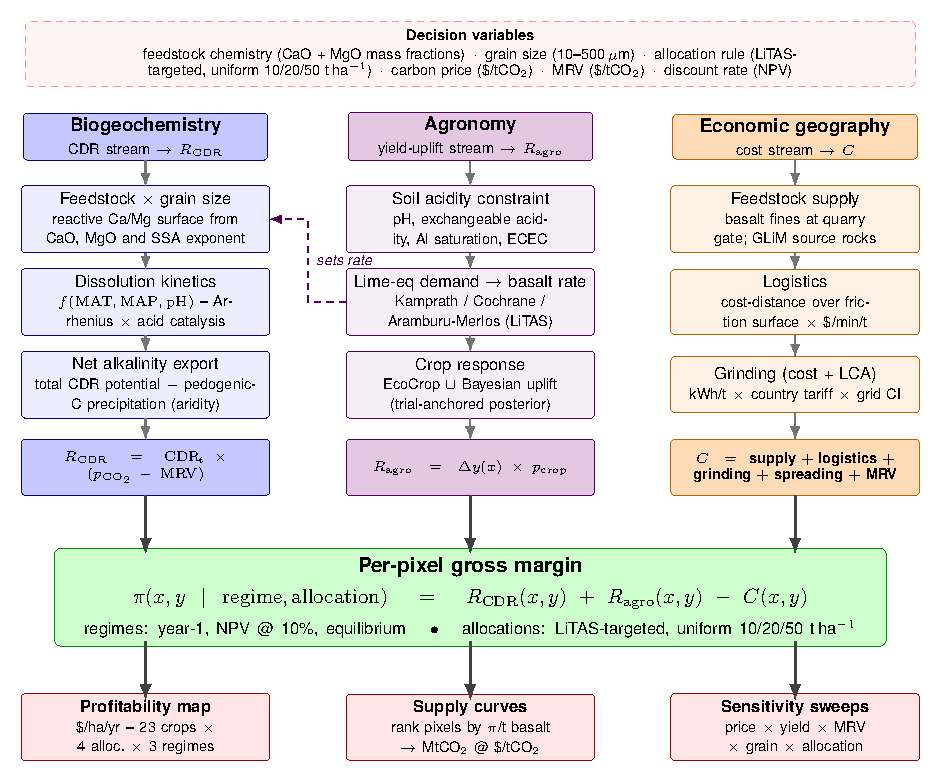
\includegraphics[width=1\linewidth,height=\textheight,keepaspectratio]{erw-conceptual-framework.pdf}
\caption{\textbf{Figure 1.} The conceptual framework. Three streams
(left to right: \emph{biogeochemistry} → carbon revenue; \emph{agronomy}
→ yield revenue; \emph{economic geography} → total cost) converge on a
single per-pixel gross- margin equation. The six dashed boxes at the top
are the user-settable decision dials. The three coloured boxes at the
bottom are the three outputs the model produces. The dashed arrow from
agronomy back to biogeochemistry captures the fact that the same basalt
application rate that the farmer needs for soil-acidity reasons is the
basalt that the biogeochemical chain dissolves to remove
CO₂.}\label{fig:framework}
\end{figure}

The three chains are:

\subsection{\texorpdfstring{4.1 The \textbf{biogeochemistry chain}
(carbon side, blue in Figure
1)}{4.1 The biogeochemistry chain (carbon side, blue in Figure 1)}}\label{the-biogeochemistry-chain-carbon-side-blue-in-figure-1}

This is the chain that tells us \textbf{how much CO₂ a tonne of basalt
will actually remove} when it sits on a particular farmer's field for a
year. The chemistry, summarised by Hartmann and colleagues {[}4{]}, says
that when basalt dissolves in moist soil, the calcium and magnesium in
the rock combine with atmospheric CO₂ to form \emph{bicarbonate}, which
then washes into rivers and eventually to the ocean, where it stays for
tens of thousands of years.

Three things determine how much of this actually happens on a given
field:

\begin{enumerate}
\def\labelenumi{\arabic{enumi}.}
\tightlist
\item
  \textbf{What's in the rock} (its calcium and magnesium content,
  default 10 \% CaO and 7 \% MgO by mass, and how finely it is ground
  --- a finer grind exposes more surface to the soil water and dissolves
  faster {[}3, 11{]}).
\item
  \textbf{The climate} (the rock dissolves faster in warm, wet
  conditions --- our reference point is a temperate American climate of
  11 °C mean annual temperature and 1000 mm mean annual precipitation,
  anchored to the Lewis et al.~{[}11{]} basalt-weathering calibration;
  tropical sites typically dissolve 1.5 to 2 times faster).
\item
  \textbf{The local soil pH} (the more acidic the soil, the faster the
  rock dissolves --- this is the chemistry of acid-catalysed weathering,
  peaking near pH 5).
\end{enumerate}

We also subtract a \textbf{pedogenic-carbonate} deduction --- a fancy
name for the well-known fact that in dry regions, some of the alkalinity
the rock releases doesn't make it to the ocean. It precipitates as solid
carbonate right there in the soil, which doesn't count as a permanent
carbon removal. We use the aridity bands keyed on mean annual
precipitation from the UNEP World Atlas of Desertification {[}12{]};
this deduction can take away as much as 90 \% of the gross removal in
arid pixels.

The output of this chain is the \textbf{CDR yield surface}: for every 1
km² patch, the tonnes of CO₂ that one hectare of treated cropland would
remove, accounting for climate, pH, and aridity penalties.

\subsection{\texorpdfstring{4.2 The \textbf{agronomy chain} (yield side,
purple in Figure
1)}{4.2 The agronomy chain (yield side, purple in Figure 1)}}\label{the-agronomy-chain-yield-side-purple-in-figure-1}

This chain tells us \textbf{how much extra crop the farmer will harvest}
if they apply basalt. The mechanism is almost the same as agricultural
lime: the dissolved cations from the rock raise the soil pH and free up
nutrients, particularly phosphorus and the basic cations themselves.

Three things determine the yield gain:

\begin{enumerate}
\def\labelenumi{\arabic{enumi}.}
\tightlist
\item
  \textbf{How acidic the starting soil is} --- the soil pH, exchangeable
  acidity, and aluminium saturation rasters come from SoilGrids-Africa
  {[}13{]}. On a soil already at pH 7, basalt does very little for the
  yield; on a soil at pH 5.0, it can do a great deal.
\item
  \textbf{The crop being grown} --- maize is moderately acid-sensitive,
  so it responds strongly; cassava is acid-tolerant, so it responds
  less. We have 23 crops mapped across Africa using the SPAM database
  {[}17{]}.
\item
  \textbf{How much rock you apply} --- we use the \texttt{limer} R
  package {[}14{]} to compute the \emph{lime-equivalent} requirement
  using the LiTAS recipe of Aramburu Merlos et al.~{[}15{]}, then
  convert lime-equivalent demand to a basalt application rate using the
  rock's chemistry. That same rate is what feeds into the
  biogeochemistry chain (this is the dashed cross-arrow in Figure 1).
\end{enumerate}

The yield gain is then multiplied by the local crop price (taken from
the United Nations FAOSTAT producer-price database, 2016--2020 average)
to give the \textbf{yield revenue surface}: dollars per hectare per year
of agronomic benefit.

\subsection{\texorpdfstring{4.3 The \textbf{economic-geography chain}
(cost side, orange in Figure
1)}{4.3 The economic-geography chain (cost side, orange in Figure 1)}}\label{the-economic-geography-chain-cost-side-orange-in-figure-1}

This chain tells us \textbf{how much it actually costs} to put a tonne
of basalt on a farmer's field. The cost has four components:

\begin{enumerate}
\def\labelenumi{\arabic{enumi}.}
\tightlist
\item
  \textbf{Buying the rock from the quarry} --- typically \$10 per tonne,
  because basalt fines (the pieces too small to use as construction
  aggregate) are a by-product that quarries are happy to sell cheap. We
  use the Global Lithological Map of Hartmann and Moosdorf {[}20{]} to
  find where basalt outcrops actually are.
\item
  \textbf{Transporting the rock from the quarry to the farm} --- this is
  by far the most variable component. A farmer 50 km from a basalt
  quarry pays a few dollars; a farmer 500 km from one pays much more. We
  calculate this using the \emph{cost-distance} over a 1-km global
  friction surface from the Malaria Atlas Project {[}19{]}, which knows
  the locations of roads, rivers, and rough terrain. The default haulage
  cost is \$0.04 per minute per tonne (a 30-tonne truck at \$80 per
  hour); we cap the haul at 1000 km because beyond that the diesel
  lifecycle emissions of the truck erase the CDR credit.
\item
  \textbf{Grinding the rock fine enough to dissolve} --- this is an
  electricity cost, so it varies by country (industrial electricity
  tariffs in Sub-Saharan Africa range roughly \$0.05 to \$0.20 per kWh).
\item
  \textbf{Spreading the rock on the field} (\$8 per tonne) and
  \textbf{measuring/verifying the CDR for the carbon market} (\$30 per
  tonne of CO₂ removed).
\end{enumerate}

The output of this chain is the \textbf{delivered cost surface}: dollars
per tonne of basalt that arrives at a farmer's field.

\subsection{4.4 Where the three chains
meet}\label{where-the-three-chains-meet}

The three chains all produce numbers in the same units (US dollars per
hectare per year, on the same 1 km² grid). The model simply adds the two
revenue streams and subtracts the cost stream to get a single
profitability map. That is equation (1) in the working paper; for this
tutorial, the words above are the equation.

\subsection{4.5 The six ``dials'' at the top of Figure
1}\label{the-six-dials-at-the-top-of-figure-1}

The boxed items at the top of Figure 1 are the \textbf{decision
variables} --- the things the user can change before running the model.
They are:

\begin{enumerate}
\def\labelenumi{\arabic{enumi}.}
\tightlist
\item
  \textbf{The chemistry of the rock} (a richer-in-calcium rock removes
  more carbon per tonne).
\item
  \textbf{How finely the rock is ground} (a finer grind dissolves faster
  but costs more electricity to produce).
\item
  \textbf{Where on the landscape we apply it} (``targeted'' --- only on
  farms where the soil acidity is high enough to need it; or ``uniform''
  --- everywhere, regardless of acidity).
\item
  \textbf{The carbon price} in dollars per tonne CO₂.
\item
  \textbf{The MRV cost} (measurement, reporting, verification --- what
  we pay to convince the carbon market that the removal actually
  happened).
\item
  \textbf{The discount rate} (how much we prefer dollars now over
  dollars in five years).
\end{enumerate}

By running the model with different settings of these dials, we can
produce supply curves and sensitivity charts (the two outputs on the
right of Figure 1) that tell us, for example, \emph{``at \$80 per tonne
of CO₂ and a 200 µm grind, the model predicts 12 million hectares are
deployable''}.

\section{5. The modelling tasks, in plain
language}\label{the-modelling-tasks-in-plain-language}

The model is built as a pipeline of \textbf{nine functional blocks},
each doing one well-defined job. Figure 2 shows how they connect. Below
I walk through each one in plain English.

\begin{figure}
\centering
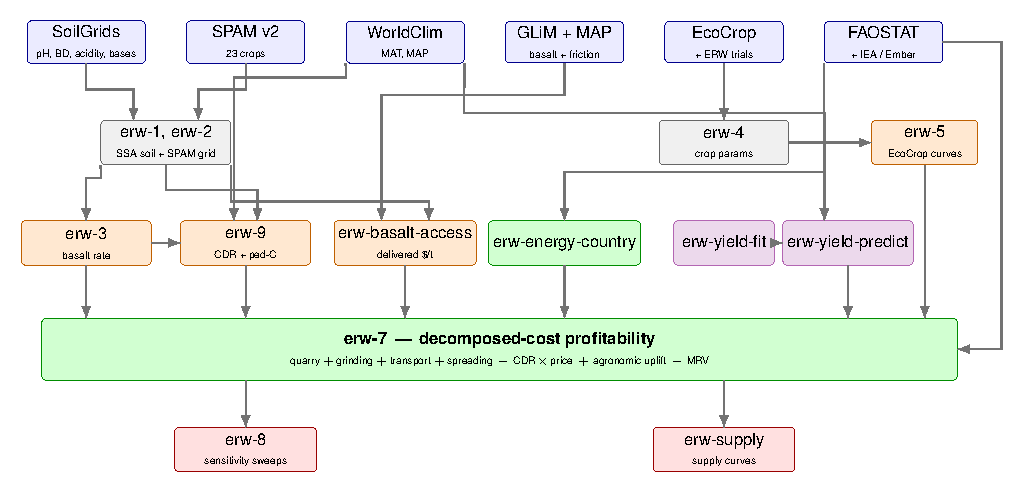
\includegraphics[width=1\linewidth,height=\textheight,keepaspectratio]{erw-pipeline-flow.pdf}
\caption{\textbf{Figure 2.} The pipeline architecture. Blue boxes are
raw data sources; grey boxes are the working-grid step; orange boxes are
geospatial processing; green boxes are economic; purple boxes are the
Bayesian-statistics step; the wide green bar in the middle is the
profitability function; the red boxes at the bottom are the
deliverables. Every arrow is a data dependency: the box at the tail of
the arrow produces something that the box at the head of the arrow
consumes.}\label{fig:pipeline}
\end{figure}

\subsection{Block 1 --- Build the working
map}\label{block-1-build-the-working-map}

We take 47 country boundaries from GADM v4, the SoilGrids-Africa
database {[}13{]} (which gives us soil pH, density, and chemistry at
every kilometre on the continent), and the MapSPAM crop-production
database {[}17{]} (which tells us where which of 23 crops is actually
being grown in Africa). We put all of these on a common grid at roughly
9 km resolution. Every subsequent step operates on this same grid.

\subsection{Block 2 --- Figure out how much rock each pixel
needs}\label{block-2-figure-out-how-much-rock-each-pixel-needs}

For every patch of cropland, we use the standard agricultural
lime-requirement formulas (the same ones a soil-testing lab would use),
implemented in the \texttt{limer} R package {[}14{]}, with the LiTAS
recipe of Aramburu Merlos et al.~{[}15{]} as the default. We then
convert that lime requirement to a basalt requirement, using the rock's
chemistry (default 10 \% CaO + 7 \% MgO by mass, with a Lewis-2021
{[}11{]} reactive-fraction calibration of 0.20 at the reference grain ×
climate). This gives us a \textbf{basalt application rate} in tonnes per
hectare for every patch.

\subsection{Block 3 --- Compute the CDR
yield}\label{block-3-compute-the-cdr-yield}

For every patch, we take the per-tonne carbon-removal potential of the
chosen rock (computed from its calcium and magnesium content), multiply
it by the climate factor (warmer-and-wetter sites dissolve the rock
faster), multiply by the pH factor (acidic soils dissolve the rock
faster), and subtract the pedogenic-carbonate fraction (the fraction of
alkalinity that gets locked up locally and never makes it to the ocean).
The result is the \textbf{tonnes of CO₂ removed per hectare per year}
for that patch, under our default assumptions.

\subsection{Block 4 --- Compute the delivered rock
price}\label{block-4-compute-the-delivered-rock-price}

This is the trickiest geospatial step. For every patch of cropland, we
ask: \emph{what is the nearest basalt outcrop, and how many minutes of
truck-time away is it?} We use the Global Lithological Map {[}20{]} for
the location of basalt outcrops and the Malaria Atlas Project 2019
motorised friction surface {[}19{]} for the per-pixel travel speed (it
accounts for roads, terrain, water bodies). The cost-distance is
accumulated using terra's algorithm; multiplying by the hourly cost of a
truck (\$80 per hour for a 30-tonne diesel truck) gives us the
\textbf{delivered price} of a tonne of basalt at every cropland pixel.

\subsection{Block 5 --- Country-resolved
electricity}\label{block-5-country-resolved-electricity}

For every country in Sub-Saharan Africa, we have a tabulated industrial
electricity price (sourced from IEA, Ember, and GET.invest 2022--2024
data, so we know what it would cost to grind a tonne of rock there) and
a tabulated grid carbon intensity (so we know how much CO₂ the grinding
emits, which we have to subtract from the gross CDR to be honest about
the net climate benefit).

\subsection{Block 6 --- Crop response}\label{block-6-crop-response}

The trickiest \emph{biological} step. We have two ways to predict how
much extra crop a farmer will get from a basalt application. The first
is \textbf{EcoCrop} --- a long-established suitability model that gives
a 0-1 score for every crop on every soil, available in R as the
\texttt{Recocrop} package by Hijmans and Manners {[}16{]}. The second is
a \textbf{Bayesian hierarchical statistical model}, implemented in
\texttt{brms} {[}18{]} and fitted to a small set of published ERW field
trials (currently 14 rows). The Bayesian model is more flexible because
it lets us update our predictions as new field trials are published. The
profitability block uses the Bayesian model when it has run; otherwise
it falls back on EcoCrop.

\subsection{Block 7 --- The profitability
function}\label{block-7-the-profitability-function}

This is the block that brings together everything above. It applies the
gross-margin equation to every patch of cropland, for every crop, for
every choice of \emph{how much rock} (targeted vs uniform 10, 20, 50
tonnes per hectare), and for every choice of \emph{time horizon}
(year-1, ten-year net-present value at 10 \% discount, or equilibrium).
The output is a large stack of map layers --- 276 of them per run: 23
crops × 4 allocation rules × 3 regimes. Default policy parameters:
carbon price \$150/tCO₂ (the 2024--25 mid-market for verified ERW
credits), MRV cost \$30/tCO₂, discount rate 10 \% per year, CDR phasing
30/25/20/15/10 \% over five years.

\subsection{Block 8 --- The supply
ranking}\label{block-8-the-supply-ranking}

In practice, basalt supply is constrained. We can't quarry an infinite
amount of basalt overnight, and we can't grind it instantly. So the
supply block ranks every patch of cropland from ``best dollar of value
per tonne of basalt'' to ``worst dollar of value per tonne of basalt'',
and produces a \textbf{supply curve}: how many tonnes of CO₂ would we
remove each year if our annual basalt supply were 1, 5, 10, 50, 250, or
500 million tonnes? This is the headline answer for an investor:
\emph{for \$X per year of basalt supply, you get Y million tonnes of CO₂
per year removed at a marginal price of \$Z per tonne}.

\subsection{Block 9 --- Sensitivity
sweeps}\label{block-9-sensitivity-sweeps}

Finally, we run the whole pipeline five times under different
assumptions, to see which of our assumptions matter most for the answer.
The five sweeps are: across different crop, basalt, and carbon prices;
across different yield-uplift levels; across different MRV costs; across
different grain sizes; and across different allocation rules.

\section{6. What the maps look like}\label{what-the-maps-look-like}

To make the model concrete, we have rendered twelve ``indicator maps''
that show the inputs and intermediate outputs across Sub-Saharan Africa.
Below are three of the most diagnostic ones.

\begin{figure}
\centering
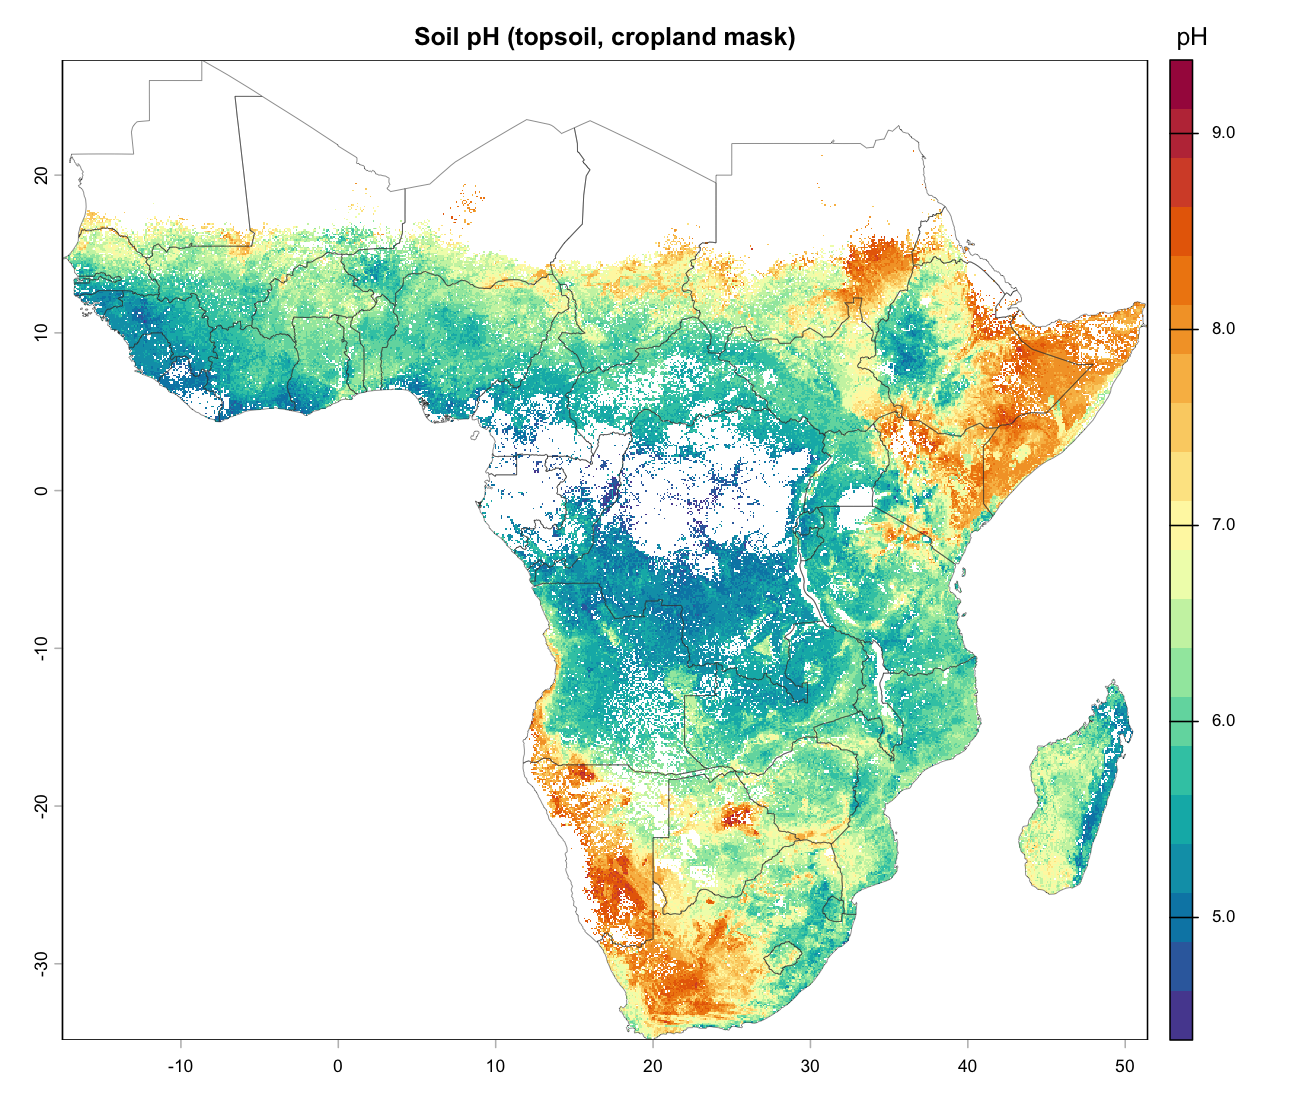
\includegraphics[width=0.8\linewidth,height=\textheight,keepaspectratio]{maps/01-soil-ph.png}
\caption{\textbf{Figure 3.} Soil pH across Sub-Saharan African cropland.
The humid-tropical zones (West Africa, the Congo basin, East Africa)
have acidic soils (orange-to-red); the Sahel and parts of southern
Africa have alkaline soils (blue). The acidic zones are where the
agronomic benefit of basalt is large.}
\end{figure}

\begin{figure}
\centering
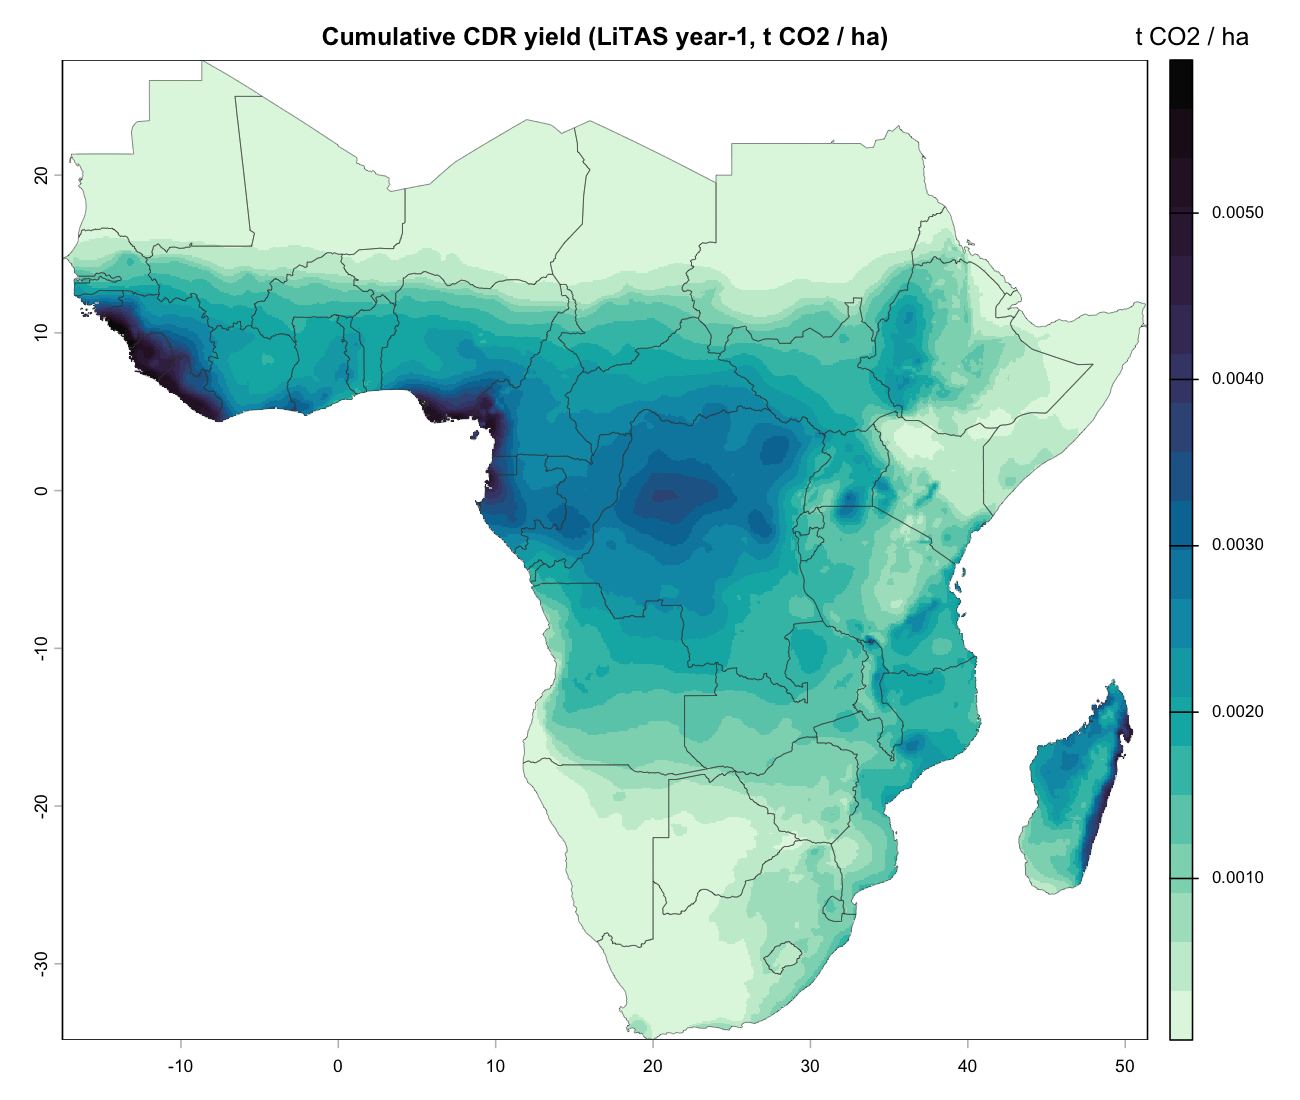
\includegraphics[width=0.8\linewidth,height=\textheight,keepaspectratio]{maps/04-cdr-yield-merlos.png}
\caption{\textbf{Figure 4.} Cumulative CDR yield --- tonnes of CO₂
removed per hectare under a one-year LiTAS-targeted basalt application.
Strongest in the humid tropics (the dark zones in the Congo basin and
around the African Great Lakes); suppressed in arid regions because the
pedogenic-carbonate deduction is large there.}
\end{figure}

\begin{figure}
\centering
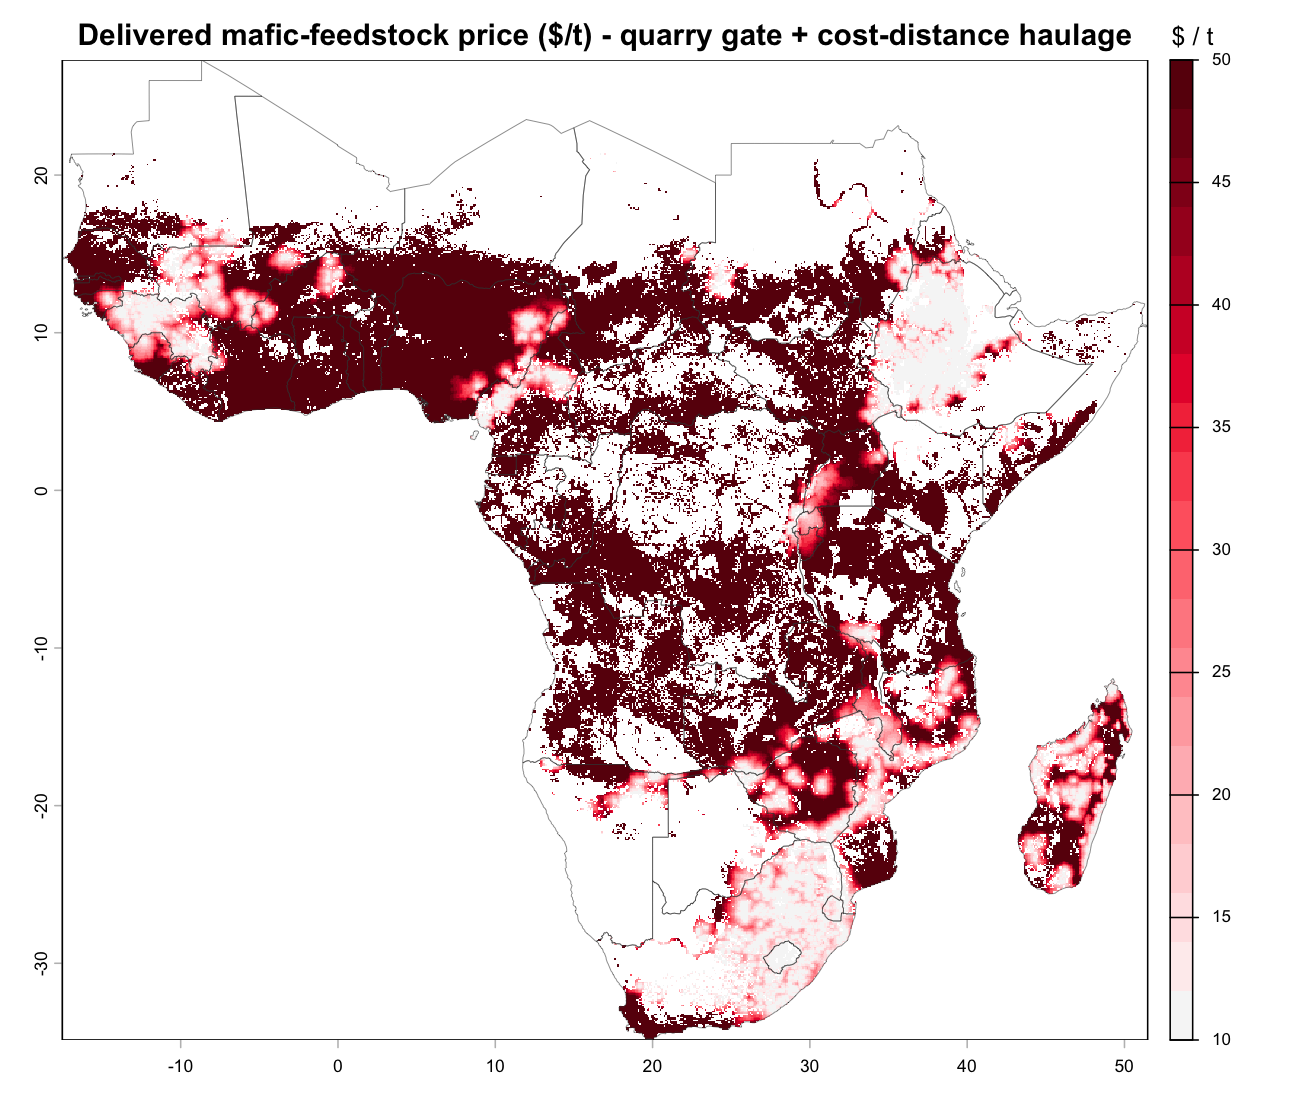
\includegraphics[width=0.8\linewidth,height=\textheight,keepaspectratio]{maps/11-basalt-delivered-price.png}
\caption{\textbf{Figure 5.} Delivered basalt price (\$ per tonne) ---
the quarry-gate price plus the cost of trucking the rock to the field.
The dark zones (cheap) are near basalt outcrops in the Ethiopian
highlands, the East African Rift, the Cameroon volcanic line,
Madagascar, and southern Africa. The light zones (expensive --- the \$50
/ tonne cap binds) are West Africa and the Sahel, where the nearest
basalt is hundreds of kilometres away.}
\end{figure}

\section{7. What we have actually produced so
far}\label{what-we-have-actually-produced-so-far}

By \textbf{2026-05-16}, the model is in the following state:

\begin{itemize}
\tightlist
\item
  All five of the input-and-surface blocks (1, 2, 3, 4, 5) have been run
  end-to-end on real data and produce the maps above.
\item
  The pH map matches the qualitative geography of African soils that you
  would expect from any soil-science textbook.
\item
  The CDR yield map peaks in the humid tropics, exactly where the
  literature {[}2, 5{]} says it should.
\item
  The delivered-basalt-price map ranges from \$10 per tonne (right at
  the outcrop) to \$50 per tonne (the cap), with about half of
  Sub-Saharan-African cropland binding at the cap. This is a strong
  signal that \emph{which country a farm is in} matters far more for ERW
  economics than the literature's standard ``uniform \$30 per tonne''
  assumption used by Renforth {[}9{]} and similar global-scale work.
\item
  Block 6's Bayesian-yield arm is \textbf{not yet fitted} --- the
  Bayesian-statistics software has to be installed and run on the
  curated trial dataset. EcoCrop is in place as the fallback.
\item
  Block 7 (the profitability function), Block 8 (supply ranking), and
  Block 9 (sensitivity sweeps) \textbf{have not yet been run}. All their
  \emph{inputs} are ready; what is left is to execute the run.
\end{itemize}

\subsection{7.1 Key constants and their
sources}\label{key-constants-and-their-sources}

Every parameter the model uses can be re-set. The defaults below are
chosen to match the central tendency of the published ERW literature.
Numbers in square brackets refer to the References section (§10).

\begin{longtable}[]{@{}
  >{\raggedright\arraybackslash}p{(\linewidth - 4\tabcolsep) * \real{0.3333}}
  >{\raggedright\arraybackslash}p{(\linewidth - 4\tabcolsep) * \real{0.3333}}
  >{\raggedright\arraybackslash}p{(\linewidth - 4\tabcolsep) * \real{0.3333}}@{}}
\toprule\noalign{}
\begin{minipage}[b]{\linewidth}\raggedright
Parameter
\end{minipage} & \begin{minipage}[b]{\linewidth}\raggedright
Default value
\end{minipage} & \begin{minipage}[b]{\linewidth}\raggedright
Source / justification
\end{minipage} \\
\midrule\noalign{}
\endhead
\bottomrule\noalign{}
\endlastfoot
Reference temperature \(T_\text{ref}\) & 11 °C & US Corn-Belt anchor
used by Lewis et al.~{[}11{]} \\
Reference precipitation \(P_\text{ref}\) & 1000 mm & as above
{[}11{]} \\
Reactive fraction at reference & 0.20 & calibrated by Lewis et
al.~{[}11{]} \\
Grain-size exponent \(\beta\) & 0.5 & surface-area scaling (Strefler et
al.~{[}3{]}) \\
Grinding-energy exponent \(\alpha\) & 1.2 & Strefler et al.~{[}3{]} \\
Pedogenic-carbonate fraction & MAP-binned 0--90 \% & UNEP aridity bands
{[}12{]} \\
Feedstock chemistry (CaO, MgO) & 10 \% CaO, 7 \% MgO & typical mafic
basalt; user-settable \\
Default grain size & 100 µm & mid-range of published ERW trials \\
Quarry-gate basalt price & \$10 / t & basalt fines as quarry by-product
(industry data) \\
Truck haulage & \$0.04 / min / t & 30-t truck @ \$80 / hour (industry
data) \\
Maximum haul distance & 1000 km & beyond cap, truck-diesel LCA erases
the credit \\
Friction surface & MAP 2019 motorised & Weiss et al.~{[}19{]} \\
On-farm spreading & \$8 / t & industry data \\
Carbon price & \$150 / tCO₂ & 2024--25 mid-market for verified ERW
credits \\
MRV cost & \$30 / tCO₂ & sampling + lab + verification + registry
(industry data) \\
Discount rate (NPV) & 10 \% / yr & conventional infrastructure rate \\
CDR realisation phasing & 30 / 25 / 20 / 15 / 10 \% over 5 yr & trial
data {[}5{]} \\
\end{longtable}

\section{8. Scope of the current work}\label{scope-of-the-current-work}

To set expectations clearly, the model in its current state covers:

\begin{itemize}
\tightlist
\item
  \textbf{Geographic scope.} 47 Sub-Saharan African countries, masked to
  QED cropland; northern boundary at the southern edge of the Sahara (so
  Morocco, Algeria, Tunisia, Libya, and Egypt are excluded); Madagascar
  is included. Working resolution ≈9 km (0.083°).
\item
  \textbf{Crops.} The 23 SPAM v2 crops {[}17{]} that cover ≥95 \% of
  African harvested area.
\item
  \textbf{Feedstock.} Mafic silicate rocks: basalt-equivalent (GLiM
  classes basic volcanic, pyroclastic, and basic plutonic / gabbro
  {[}20{]}). All other feedstock classes --- ultramafics, wollastonite,
  steel slag, cement-kiln dust, mine tailings --- are out of scope (see
  Limitations below).
\item
  \textbf{Time horizons.} Year-1 only; ten-year net-present value at 10
  \% discount; equilibrium (saturating CDR). All three run in parallel.
\item
  \textbf{Allocation rules.} Four --- LiTAS-targeted (apply only where
  soil acidity is high enough to need it) plus uniform 10, 20, and 50
  t/ha.
\item
  \textbf{Decision variables.} Six dials (feedstock chemistry, grain
  size, allocation rule, carbon price, MRV cost, discount rate) --- see
  §4.5.
\end{itemize}

\section{9. Limitations of the current
work}\label{limitations-of-the-current-work}

Six substantive limitations should be named upfront. They are listed in
rough order of how much they constrain the current results.

\begin{enumerate}
\def\labelenumi{\arabic{enumi}.}
\tightlist
\item
  \textbf{The feedstock catalogue is incomplete.} The model currently
  considers only basalt-and-gabbro outcrops from GLiM v1 {[}20{]}. The
  literature recognises four additional candidate feedstock classes:
  ultramafic silicates (excluded for cropland use because of Ni/Cr
  leaching risk --- see Vienne et al.~{[}10{]} and Beerling et
  al.~{[}2{]}), calcium-silicate by-products (wollastonite, steel slag,
  cement-kiln dust), construction by-products (recycled concrete fines,
  fly ash), and mine tailings. The omission of industrial alkaline
  by-products in particular materially shifts the picture for countries
  with no mafic outcrops --- much of West Africa, where the model
  currently predicts delivered prices at the \$50/tonne cap.
\item
  \textbf{The Bayesian yield-uplift arm is fitted on a small trial
  dataset} --- currently 14 trial rows from the published ERW
  literature. The posterior is therefore prior-dominated. The Bayesian
  framework is correct (it grows in evidence weight as data is added),
  but quantitative yield predictions today carry wide uncertainty. The
  2024 US Corn-Belt trial {[}5{]}, the 2024--25 Kisumu trial {[}6{]},
  and the 2025 Swiss-vineyard trial {[}7{]} are all candidates for
  incorporation into the next iteration.
\item
  \textbf{The full profitability run is not yet executed.} Blocks 7, 8,
  and 9 (profitability, supply-constrained ranking, sensitivity sweeps)
  have not yet been run end-to-end. All their inputs are in place; what
  remains is to execute the run and publish the resulting profitability
  maps and supply curves.
\item
  \textbf{The aridity proxy is rough.} The pedogenic-carbonate deduction
  currently uses mean annual precipitation (MAP) alone, binned into
  UNEP-1992 categories {[}12{]}. The literature standard is the full
  aridity index \(\text{AI} = \text{MAP} / \text{PET}\), which requires
  a potential-evapotranspiration surface from CGIAR-CSI or computed from
  WorldClim minimum-and-maximum temperatures. We expect this to be a
  small-effort, moderate-payoff upgrade.
\item
  \textbf{MRV cost is a single flat number.} \$30/tCO₂ for all pixels
  and all protocols is a strong simplification. In practice MRV cost is
  scale-dependent and protocol-dependent (Isometric vs Puro vs others),
  and is materially higher in smallholder-dominated systems where
  sampling has to be coordinated across many small farms. The
  sensitivity sweep over MRV \$0--80/tCO₂ in Block 9 partly bounds this,
  but a proper treatment is a future revision.
\item
  \textbf{The model is per-pixel and farmer-perspective.} A complete
  economic model of deployment would also incorporate aggregator-level
  economics: pooling MRV across many small farms, finance for
  distributed deployment, and coordination with carbon-market
  intermediaries. These are likely material at the scale of
  smallholder-dominated cropping in Sub-Saharan Africa.
\end{enumerate}

A seventh, more technical caveat: the SoilGrids-Africa pH raster
{[}13{]} is itself a machine-learning prediction with its own
uncertainty, which the current model treats as deterministic. Future
work could propagate that uncertainty into the gross-margin map using
the Bayesian framework already in place for the yield-uplift arm.

\section{10. References}\label{references}

The default constants and the framing of the conceptual model rest on a
specific set of published references. All entries below have been
verified against the published record.

{[}1{]} IPCC (2023). \emph{Climate Change 2023: Synthesis Report.} Sixth
Assessment Report of the IPCC, Geneva.
\url{https://www.ipcc.ch/report/ar6/syr/}.

{[}2{]} Beerling, D. J. et al.~(2020). Potential for large-scale CO₂
removal via enhanced rock weathering with croplands. \emph{Nature} 583,
242--248. doi:10.1038/s41586-020-2448-9.

{[}3{]} Strefler, J., Amann, T., Bauer, N., Kriegler, E., Hartmann, J.
(2018). Potential and costs of carbon dioxide removal by enhanced
weathering of rocks. \emph{Environmental Research Letters} 13, 034010.
doi:10.1088/1748-9326/aaa9c4.

{[}4{]} Hartmann, J. et al.~(2013). Enhanced chemical weathering as a
geoengineering strategy. \emph{Reviews of Geophysics} 51, 113--149.
doi:10.1002/rog.20004.

{[}5{]} Beerling, D. J. et al.~(2024). Enhanced weathering in the US
Corn Belt delivers carbon removal with agronomic benefits. \emph{PNAS}
121 (9), e2319436121. doi:10.1073/pnas.2319436121.

{[}6{]} Haque, F. et al.~(2025). \emph{Agronomic Performance of Enhanced
Rock Weathering in a Tropical Smallholder System: A Maize Trial in
Kenya.} CDRXIV preprint 410 (Flux Carbon / UNCCD pilot).
\url{https://cdrxiv.org/preprint/410}.

{[}7{]} Dupla, X., Bertagni, M. B., Grand, S. (2025). Three Years of
Field Trials Indicate a Sustained Enhanced Rock Weathering Signal with
Limited CO₂ Removal. \emph{Environmental Science \& Technology} 59 (48),
25751--25764. doi:10.1021/acs.est.5c09820.

{[}8{]} Kanzaki, Y. et al.~(2024). \emph{Soil cation storage as a key
control on the timescales of CDR through enhanced weathering.} ESS Open
Archive preprint, doi:10.22541/essoar.170960101.14306457/v1.

{[}9{]} Renforth, P. (2019). The negative emission potential of alkaline
materials. \emph{Nature Communications} 10, 1401.
doi:10.1038/s41467-019-09475-5.

{[}10{]} Vienne, A. et al.~(2022). Enhanced weathering using basalt rock
powder: carbon sequestration, co-benefits and risks in a mesocosm study
with \emph{Solanum tuberosum}. \emph{Frontiers in Climate} 4, 869456.
doi:10.3389/fclim.2022.869456.

{[}11{]} Lewis, A. L. et al.~(2021). Effects of mineralogy, chemistry
and physical properties of basalts on carbon capture potential and
plant-nutrient element release via enhanced weathering. \emph{Applied
Geochemistry} 132, 105023. doi:10.1016/j.apgeochem.2021.105023.

{[}12{]} Middleton, N. \& Thomas, D. S. G. (eds.) (1992). \emph{World
Atlas of Desertification.} United Nations Environment Programme, London.

{[}13{]} Hengl, T. et al.~(2017). SoilGrids250m: Global gridded soil
information based on machine learning. \emph{PLOS One} 12 (2), e0169748.
doi:10.1371/journal.pone.0169748.

{[}14{]} Aramburu Merlos, F. (2022). \emph{limer: Acidic soil management
for agriculture.} R package, GAIA Africa.
\url{https://github.com/gaiafrica/limer}.

{[}15{]} Aramburu Merlos, F., Silva, J. V., Baudron, F., Hijmans, R. J.
(2023). Estimating lime requirements for tropical soils: Model
comparison and development. \emph{Geoderma} 432, 116421.
doi:10.1016/j.geoderma.2023.116421.

{[}16{]} Hijmans, R. J. \& Manners, R. (2025). \emph{Recocrop:
Estimating Environmental Suitability for Plants.} R package version
0.4-2, CRAN. doi:10.32614/CRAN.package.Recocrop.

{[}17{]} You, L. et al.~\emph{MapSPAM --- Spatial Production Allocation
Model.} IFPRI and HarvestChoice. Used here via
\texttt{geodata::crop\_spam}: SPAM 2010 V2.0 globally and SPAM 2017-SSA
for Africa. \url{https://www.mapspam.info}.

{[}18{]} Bürkner, P.-C. (2017). brms: An R package for Bayesian
multilevel models using Stan. \emph{Journal of Statistical Software} 80
(1), 1--28. doi:10.18637/jss.v080.i01.

{[}19{]} Weiss, D. J. et al.~(2020). Global maps of travel time to
healthcare facilities. \emph{Nature Medicine} 26, 1835--1838.
doi:10.1038/s41591-020-1059-1. (The motorised friction surface, nominal
year 2019, is derived from this work.)

{[}20{]} Hartmann, J. \& Moosdorf, N. (2012). The new global
lithological map database GLiM. \emph{Geochemistry, Geophysics,
Geosystems} 13, Q12004. doi:10.1029/2012GC004370. Dataset DOI:
10.1594/PANGAEA.788537.

\section{11. What this tutorial does and does not
cover}\label{what-this-tutorial-does-and-does-not-cover}

This tutorial covers the \textbf{conceptual and modelling tasks}: what
the model is, how it works, what it produces, and where its limits are.

It does \textbf{not} cover the day-to-day implementation details: the R
scripts, the data-handling, the rebuilding of the figures, the
TikZ/LaTeX setup. Those are described in the companion document
\emph{Ex-Ante ERW Model --- Living Documentation}
(\texttt{docs/erw-model.pdf}). The more academic write-up is the
\emph{Working Paper} (\texttt{docs/erw-working-paper.pdf}), which
contains the formal equations and the full reference list with author
lists.

\section{12. Glossary}\label{glossary}

\textbf{Allocation rule} --- How we decide which fields get basalt.
Either \emph{LiTAS-targeted} (only fields where the soil acidity is high
enough to benefit) or \emph{uniform 10 / 20 / 50 tonnes per hectare}
(everywhere, regardless of acidity).

\textbf{Basalt} --- A common, dark, fine-grained volcanic rock rich in
calcium and magnesium. The most-studied feedstock for enhanced rock
weathering on cropland.

\textbf{Bayesian hierarchical model} --- A statistical model that
combines prior beliefs about parameters with observed data to produce a
posterior distribution over the parameters. ``Hierarchical'' means the
model has random effects --- for example, a per-crop intercept that lets
each crop have its own response without forcing them all to be the same.
We use it in Block 6 to predict yield response to basalt.

\textbf{CDR} --- Carbon dioxide removal: the broad category of methods
that take CO₂ \emph{out of the atmosphere} (as opposed to merely
\emph{avoiding new emissions}).

\textbf{Cost-distance} --- A spatial-analysis technique that, instead of
measuring straight-line distance, accumulates a \emph{cost} (here:
minutes-of-travel) as you move from a source pixel. We use it to compute
how slow each kilometre of getting from a basalt quarry to a farm is,
given the local roads and terrain.

\textbf{Discount rate} --- The annual percentage by which we reduce the
value of future dollars when comparing them to today's dollars. We use
10 \% per year as a baseline.

\textbf{EcoCrop} --- A long-established crop-suitability model that
scores how suitable a given environmental condition (soil pH,
temperature, moisture) is for a given crop on a 0 to 1 scale.

\textbf{Enhanced rock weathering (ERW)} --- The deliberate spreading of
finely-ground silicate rock (in this project, basalt) on cropland to
accelerate the natural chemical weathering reactions that consume
atmospheric CO₂.

\textbf{FAOSTAT} --- The Food and Agriculture Organization's online
statistics database. We use it for crop-by-country producer prices.

\textbf{Gabbro} --- The intrusive (slower-cooled) equivalent of basalt;
chemically nearly identical. We include it in the feedstock supply
because it has the same desirable properties.

\textbf{GLiM} --- The Global Lithological Map: a worldwide map of
surface rock types, used here to find where basalt outcrops actually
are.

\textbf{Grain size} --- How finely the rock is ground. We work in
micrometres (µm). Below about 50 µm, dissolution is fast but grinding
costs jump sharply.

\textbf{Gross margin} --- In economics, total revenue minus total
variable cost. In our model, the CDR revenue plus the yield revenue
minus the delivered + on-farm cost.

\textbf{Lime-equivalent demand} --- The agronomic concept that there is
a specific quantity of agricultural lime that would, in theory, bring a
soil to its crop's optimum pH. Basalt and lime have similar mechanisms,
so we convert the lime requirement to a basalt requirement using the
rock's calcium and magnesium content.

\textbf{LiTAS} --- Lime-Targeted Application Strategy: one of the more
recent and accurate recipes for calculating the lime-equivalent demand
on tropical acid soils. Defined by Aramburu Merlos and colleagues in
2023.

\textbf{Malaria Atlas Project (MAP)} --- A research consortium that,
among other things, publishes a global 1-km ``friction surface'' that
scores how slow it is to traverse each pixel on the Earth's surface. We
use this for the cost-distance calculation in Block 4.

\textbf{MRV} --- Measurement, reporting, and verification: the protocols
that a carbon-credit buyer requires to be convinced that the carbon
removal they are paying for actually happened. Default cost in our
model: \$30 per tonne of CO₂.

\textbf{NPV} --- Net present value. The discounted sum of a stream of
future cash flows. Used here when we want to compare an ERW deployment
over a ten-year horizon to one over a single year.

\textbf{Pedogenic carbonate} --- Soil-formed carbonate. Where conditions
are arid, some of the alkalinity that the dissolving rock releases
doesn't make it to the ocean; it precipitates as solid carbonate right
in the soil. This locked-up alkalinity does not count as a permanent
carbon removal, so we subtract it.

\textbf{Pixel} --- A 1 km² (more precisely, about 0.083 ° on a side, or
roughly 9 km × 9 km after our 10-fold spatial aggregation) cell of the
working grid. Every output of the model is a per-pixel number.

\textbf{Pyroclastic} --- Volcanic rock made of fragments of pre-existing
volcanic material. In GLiM, marked \texttt{py}. Same chemistry as
basalt.

\textbf{Quarry-gate price} --- The price you pay for the rock at the
quarry gate, before transport. We use \$10 per tonne for basalt fines.

\textbf{Recocrop} --- An R-package implementation of EcoCrop, used here
for the EcoCrop-arm fall-back of Block 6.

\textbf{SoilGrids} --- A global gridded map of soil properties (pH, bulk
density, exchangeable cations, \ldots) produced by ISRIC. We use the
1-km Africa subset.

\textbf{SPAM} --- The Spatial Production Allocation Model: a global
gridded dataset of where which crops are grown, produced by the
International Food Policy Research Institute.

\textbf{Supply curve} --- A graph that shows, for each level of annual
basalt supply (in million tonnes per year), the marginal price per tonne
CO₂ at which the next tonne is removed. The standard economic output of
a deployment-ranking exercise.

\textbf{Targeted vs uniform} --- See \emph{Allocation rule}.

\textbf{Working grid} --- The common 9-km grid on which all the model's
inputs and outputs are co-registered. Built in Block 1.

\end{document}
